%! TeX program = lualatex
\documentclass[a4paper,chapter,atbegshi,]{oblivoir}
\usepackage[dbl4x6]{fapapersize}
\usepackage{amsmath,amssymb,amsfonts,mdframed,enumitem,graphicx,wrapfig,xcolor}
\usepackage{fontspec,caption,braket,twemojis,}
\usepackage{hyperref}
\hypersetup{
  colorlinks=true,
  linkcolor=teal,
  filecolor=magenta,
  urlcolor=cyan,
}
\usepackage{nicematrix}
\graphicspath{{./IMG/}}
\setlist{nosep}

\renewcommand\chaptername{강}

\makepagestyle{mystyle} 
\makeevenhead{mystyle}{\thepage}{}{\leftmark}
\makeoddhead{mystyle}{\rightmark}{}{\thepage}
\makeatletter
\makepsmarks{mystyle}{%
  \createmark{chaptername chapter}{left}{shownumber}{}{}
  \createmark{section}{right}{shownumber}{}{ }
}
\makeatother

\begin{document}
\title{양자정보학 개론\thanks{원문: \url{https://www.scottaaronson.com/qclec.pdf}}}
\author{
  스콧 애론슨\thanks{코리 오스트로브{\tiny Corey Ostrove}와 
  파울로 알브스{\tiny Paulo Alves}의 큰 도움을 받았다.}, 
    2018년 가을\\
    번역: 김태원
}
\date{\today}
\newpage
\maketitle\thispagestyle{empty}\newpage

\tableofcontents\pagestyle{mystyle}

\chapter{강의 개요 및 확장 처치-튜링 논제}
\begin{itemize}[label=\(\blacktriangleright\)]
    \item 양자정보학은 천성이 간학문적인 분야다. (물리학, 전산학, 수학, 공학, 철학)
    \item 양자정보학은 단지 유용한 장치나 알고리즘의 발명만이 아니라 양자역학적 작용의 명료화에 관한 것이기도 하다.
    \begin{itemize}
        \item 양자역학으로 할 수 있느냐 없느냐는 물음을 던지기 위한 것이자
        \item 양자역학 자체의 본성에 대한 더 나은 이해를 독려하기 위한 것이다.
    \end{itemize}
    \item 애론슨 교수는 양자정보학 연구의 이론적인 극단에 헌신한다.
    \item 이론가들은 실험가들이 만드는 것을 알리고 이는 다시 이론가들의 질문에 영향을 미친다.
\end{itemize}

\hfill

오늘은 물리적 세계에 관해 ``자명한" 진술들을 명시하겠다.
그런 다음 양자역학이 이들 진술 가운데 몇몇만 놔두고 나머지는 뒤엎어 버리는 광경을
목도할 테다. 
그런데 이들 진술 간의 차이란 종종 아주 미묘하다!
우선...\hfill\break

\begin{description}[leftmargin=0cm]
    \item[\textbf{확률}\;] 
        $(P\in[0,1])$는 세상의 불확실성을 나타내는 표준적인 방법이다. 
        확률은 아래 같은 일련의 공리를 따라야 한다.
        \begin{itemize}[label=$\blacktriangleright$]
            \item  상호배타적이며 포괄적인 사건{\footnotesize mutually exclusive
            exhaustive events} $n$개의 집합에 대해  
                확률들의 합은 $P_1+P_2+\cdots+P_n=1$을 만족한다.
            \item 임의의 사건에 대한 확률은 $P_i\geq0$을 만족한다.
        \end{itemize}
        \begin{align*}\bullet\\\bullet\\\bullet\end{align*}
\end{description}

\newpage

\hfill\parbox[t]{9cm}{\textcolor{gray}{\itshape``확률은 전부 우리 손 안에 있다"는
관점이 존재한다. 우주에 관해 전부 (요컨대 태양계 속 모든 원자의 
위치/속도를) 안다면 방정식들을 처리해서 뭐가 일어나는지 아닌지
보기만 하는 것으로 충분하다는 뜻이다.}}\break

\begin{wrapfigure}{r}{0.35\textwidth}
    \centering
    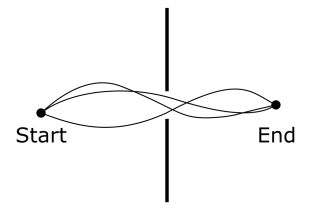
\includegraphics[width=0.35\textwidth]{iqis1_001}
\end{wrapfigure}

\hfill

장벽이 두 점을 구분하고 있다고 하자. 장벽에는 슬릿{\footnotesize slit}이 하나
있다. 우리는 입자가 한 점에서 다른 점으로 이동하는 확률을 측정하고자 한다. 
경로를 늘리면 (다시 말해 또 다른 슬릿을 개방하면) 다른 쪽에 도달할 가능성이 증가, 아니 적어도 감소하지는 않을 것은 분명하다. 확률이 \textbf{단조}{\footnotesize
monotone}라는 말로 이런 성질을 가리킬 수 있다.

\hfill
\begin{description}[leftmargin=0cm]
    \item[국소성{\footnotesize Locality}.] 
        우주를 가로지르는 전파가 특정 속도를 지닌다는 원리다.
        공간상의 한 부분에 대해 상태를 업데이트할 때는 그 부분 주변의 지식만
        필요할 것이다. 이에 적절한 모델은 콘웨이의 생명게임{\footnotesize Game Of
        Life}이다. 계{\footnotesize system}에 일으키는 변화는 계에 영향을 미칠
        수 있다. 하지만 각 칸은 오직 가장 가까운 주변부와 상호작용할 뿐이다. 
        그리하여 변화는 오직 특정 속도로 전파한다.
\end{description}

\begin{wrapfigure}{l}{0.33\textwidth}
    \centering
    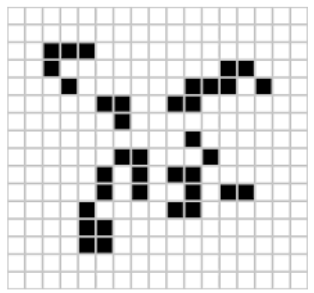
\includegraphics[width=0.33\textwidth]{iqis1_002}
\end{wrapfigure}

\hfill

국소성은 물리학에서 자연스럽게 모습을 드러낸다. 아인슈타인의 특수상대성이론
덕분이다. 이는 어떤 신호도 빛의 (유한한) 속력보다 빠르게 전파할 수 없다는
암시를 지니는 원리다. 이 간단한 원리는 여러 물리 현상을 설명할 수 있다. 
특수상대성이론에 따른 어떤 관찰자의 관점으로는 광속보다 빠르게 이동하는 것이라면
모두 사실상 시간을 역행한다.\break

\begin{description}[leftmargin=0cm]
    \item[국소적 실재론{\footnotesize Local Realism}.] 멀리 떨어진 사건에 대한
        지식의 업데이트를 몽땅 무작위 변수의 상관관계로 설명할 수 있다는
        원리다. 당신은 오스틴, 친구는 샌프란시스코에 있다고 하자. 둘 다
        같은 신문을 구독한다. 아침이 되자 당신은 신문을 펼친다. 그러자 당신의
        지식은 즉각 붕괴한다. 바로 샌프란시스코 친구가 지니는 신문의 헤드라인에
        관한 지식이었다. 붕괴의 자리에는 지금 손에 쥔 신문의 헤드라인이 들어선다.
        신문을 집기 전의 상황이라면 당신의 지식은 확률 분포로 가장 잘 서술될 수
        있었다. 하지만 지금 결과는 완벽하게 상호연관되어 있다. 그래서 신문
        헤드라인을 학습하는 바로 그 순간 친구의 신문도 동일한 헤드라인을
        지닌다고 즉각 알 수 있다.
        \end{description}

\newpage
\hfill\parbox[t]{9cm}{\textcolor{gray}{\itshape어떤 대중과학 기사는 한 입자의
스핀을 측정할 때 은하계 이면에 있는 또 다른 입자의 스핀을 즉각 알 수 있는
방법을 논한다. 다만 별다른 언급이 따로 없다면 신문 사례와 다를 바 없다.
그리고 국소적 실재론과 100\% 호환되는 것으로 보인다!}}

\hfill\break

\begin{description}[leftmargin=0cm]
    \item[처치-튜링 논제{\footnotesize Chuch-Turing Thesis}.] 처치-튜링 논제란
        모든 물리적인 과정이 튜링장치를 통해 원하는 임의의 정밀도로
        시뮬레이션 가능하다는 진술이다. 처치와 튜링은 이 진술을
        계산{\footnotesize computation}에 대한 정의로 이해했다. 그러나 이런 정의
        대신 물리 세계에 관해 반증가능한 주장으로 처치-튜링 논제를 받아들일 수
        있다. 전체 우주가 일종의 초대형 비디오 게임이라는 발상으로
        이해하는 것이다. 여기에는 쿼크와 블랙홀, 온갖 종류의 복잡한 것이라면
        뭐든 있다. 다만 종국에는 이들을 컴퓨터로 시뮬레이션할 수 있어야 한다.
        \textbf{확장 처치-튜링 논제}는 여기서 더 나아간다. 바로 디지털 컴퓨터를
        통한 실재{\footnotesize reality}의 시뮬레이션에는 시간과 공간과 여타
        계산 자원상 다항{\footnotesize polynomial}의 (즉 선형이나
        이차의) 증가가 최대라는 것이다.
\end{description}

\hfill

\hfill\parbox[t]{9cm}{\textcolor{gray}{이론전산학 수업은 근본적으로 수학 수업처럼
보일 수 있다. 그럼 뭐가 이론전산학과 실재를 연결하는가? 바로 처치-튜링 논제다.}}

\hfill\break

그렇다면 양자역학은 이들 원리에 대해 뭐라고 말하고자 하는가? 나머지 수업에 관한
예고편을 제공하자면 아래와 같다.

\hfill

\begin{itemize}[label=$\blacktriangleright$]
    \item 확률을 쓰긴 한다. 다만 \emph{연산}을 아예
        달리할 것이다. 그리고 단조의 공리를 위배하겠다. 즉 한 사건이
        일어날 수 있는 방법의 \emph{증가}에 의해 그 사건이 일어나는 확률은
        \emph{감소}할 수 있다.
    \item 국소성은 놔둔다. 그러나 \emph{국소적 실재론}은 타도하겠다. 이 두
        원리가 서로에 대한 재진술처럼 들렸다면 글쎄 양자역학은 이들 간의 차리를
        극적으로 묘사하리다!
    \item 앞으로 확인하겠지만 처치-튜링 논제는 양자역학이라는 역광에도 불구하고
        상태가 좋아 보인다. 그러나 확장 처치-튜링 논제는 그 반례로서 이글거리며
        서 있는 양자컴퓨팅 탓에 거짓으로 보인다. 양자컴퓨팅은 확장 처치-튜링 
        논제에 대해 아마 우리의 물리학 법칙들이 허용하는 단 하나의 반례일지도
        모른다. 그런데도 이야기한 김에 덧붙이자면 양자 버전으로 확장 처치-튜링
        논제를 정식화할 수도 있다. 이 양자 버전은 오늘날의 지식에 한해 아직 
        참이다.
\end{itemize}

\hfill\break

\hfill\parbox[t]{9cm}{\textcolor{gray}{\itshape확장 처치-튜링 논제에 대해 다른
반례도 생각해 볼 수 있다. 가령 어떤 이들은 시간 팽창{\footnotesize time 
dilation}을 사용하면 미래로 수십억 년을 여행해 난해한 문제들{\footnotesize hard
problems}에 대한 결과를 취할 수 있다고 제안했다. 재밌다! 하지만 \underline{엄청난}
에너지가 필요하겠다. 또 그만큼 에너지를 한 장소에 지니면 당신은 블랙홀로
붕괴한다. 별로 재미없다!}}

\hfill\break

\begin{figure}[h]
    \centering
    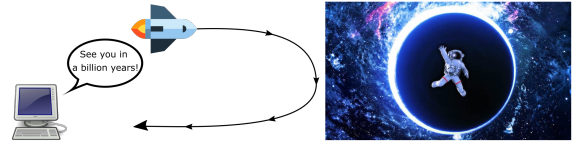
\includegraphics[width=0.9\textwidth]{iqis1_003}
\end{figure}

\chapter{확률론과 양자역학}

유명한 물리학자 리차드 파인만이 말하기를 양자역학은 전부 \textbf{이중
슬릿 실험}으로 요약할 수 있다. 이중 슬릿 실험은 좁은 슬릿 두 개가 있는
벽으로 한 번에 하나씩 광자를 쏜다. 이때 확률론적인 것은 두 번째 벽에 안착하는
광자다. 광자가 나타나는 구역을 뒷벽에 표시해 보자. 어떤 구역은 아주 그럴듯하고
어떤 구역은 그렇지 않다. 그림 \ref{fig:figure21} - \ref{fig:figure23}은 
기본 실험 구성과 단일 및 이중 슬릿 실험을 수행 결과를 보인다. 

스크린상 어떤 구역은 그럴듯하고 어떤 구역은 그럴듯하지 않다. 그런데 이 결과
자체가 기이하지는 않다. 각 광자가 (``전자태그"와 같은) 미지의 여유
자유도{\footnotesize degree of freedom}를 지녀서 작금의 현상을 결정했다는
이론으로 충분히 설명할 수 있는 결과다. 기이한 사실은 이렇다. 두 번째 벽
위 어떤 구간에 대해 광자가

\hfill

\hfill\parbox[t]{12cm}{
    두 슬릿 모두 개방된 구간에 안착하는 확률을 $P$,\\
    1번 슬릿만 개방된 구간에 안착하는 확률을 $P_1$,\\
    2번 슬릿만 개방된 구간에 안착하는 확률을 $P_2$라고 하자.}

\hfill\break

$P=P_1+P_2$라고 생각하겠지만 실험에 따르면 사실이 아니다! 모든 슬릿이 개방될 때
맞지 않은 구역이더라도 이따금 하나의 슬릿만 개방될 때 맞을 수 있다. 

\hfill

\hfill\parbox[t]{9cm}{\textcolor{gray}{\itshape ``신이 주사위를 굴린다"는 말은
별로 기이하지 않다. 차라리 기이한 쪽을 말하자면 ``이건 멀쩡한 주사위가 아니다"!}}

\newpage

\begin{figure}[ht]
    \begin{minipage}{0.48\textwidth}
    \centering
    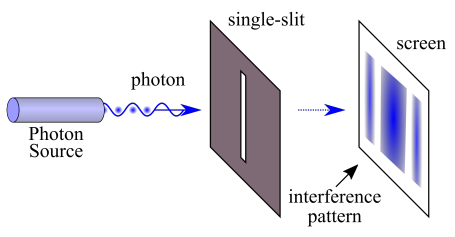
\includegraphics[width=.9\linewidth]{iqis1_004}
    \caption{\label{fig:figure21}\emph{단일 슬릿} 광자 간섭 실험 구성}
    \end{minipage}\hfill
    \begin{minipage}{0.48\textwidth}
        \centering
        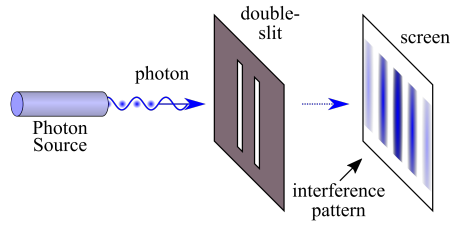
\includegraphics[width=.9\linewidth]{iqis1_005}
        \caption{\label{fig:figure22}\emph{이중 슬릿} 광자 간섭 실험 구성}
    \end{minipage}\vspace{0.25cm}
    \centering
    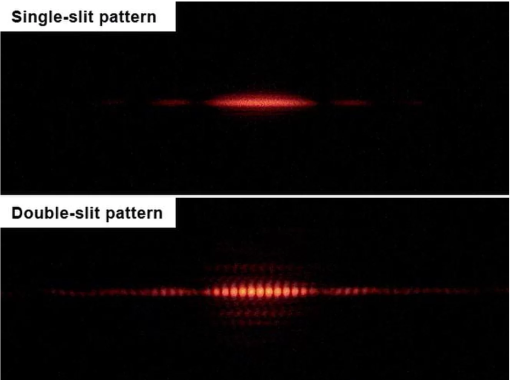
\includegraphics[width=.5\textwidth]{iqis1_006}\vspace{0.2cm}
     \caption{\label{fig:figure23}실질적인 실험으로 보이는 단일 슬릿과 이중 슬릿
    간섭 패턴의 비교다. 단일 슬릿 패턴에는 보이지 않은 신규 암점{\footnotesize
    dark spots}이 (즉 광자 안착 확률이 낮은 구역이) 이중 슬릿 패턴에 나타난다는
    사실을 확인하라.}
\end{figure}

\newpage

광자가 어느 슬릿을 지나갔는지 측정하고 싶을 수 있겠다. 하지만 그러다간 각 슬릿에
하나씩 밝은 부분이 남는 더 말이 되는 쪽으로 측정결과를 \emph{바꾸고 만다}. 
의식을 지닌 관찰자가 있는지는 중요하지 않다는 사실에 유의하라. 지나간 슬릿의
정보가 외부 환경에 아무튼 유출되면 결과는 고전 확률론을 따르는 꼴로 돌아간다. 

\hfill

\hfill\parbox[t]{9cm}{\textcolor{gray}{\itshape자연은 말하는 듯 하다. ``뭐? 나? 나 아무것도 안 했는데?''}}

\hfill

\begin{figure}[h]
  \centering
  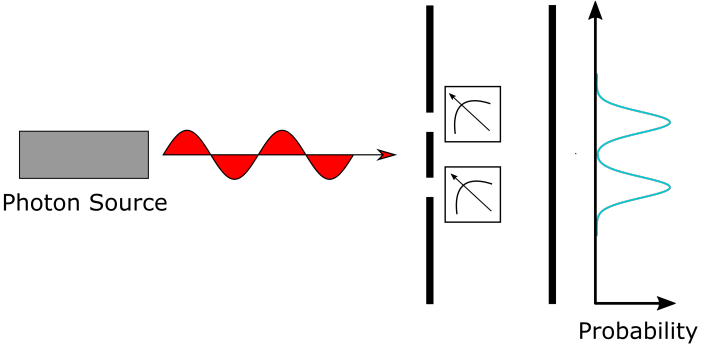
\includegraphics[width=.8\textwidth]{iqis1_007}
  \caption{\label{fig:figure24}임의의 광자가 지나가는 슬릿을 측정하는 장치로
    진행한 이중 슬릿 실험이다. 이 경우 확률 분포는 개별 단일 슬릿 분포의 평균처럼
  보인다.}
\end{figure}

이처럼 계{\footnotesize system}가 제 환경과 짝을 맺을 때 고전 확률론에 이르는
되박이{\footnotesize reversion}를 \textbf{결어긋남}{\footnotesize
decoherence}이라고 부른다. 결어긋남은 확률론 법칙이 대개 일상에서 돌아가는 듯
보이는 이유다. 고양이는 생과 사라는 두 상태의 중첩{\footnotesize
superposition}으로 나타나지 않는다. 왜냐하면 고양이는 거듭하여 제 환경과
상호작용하기 때문이다. 본질적으로 이들 상호작용은 `고양이 계'에 관한 정보를
유출한다. 양자 중첩은 제 환경에서 격리될 적의 입자 혹은 입자들의 군{\footnotesize
group}에 대해 일어나는 일이다. 입자는 격리되어야 하며 이런 당위가 바로
양자컴퓨터를 만들기 어려운 이유다.

\hfill

\hfill\parbox[t]{9cm}{\textcolor{gray}{\itshape입자들이 \underline{완벽하게}
격리되지는 않았지만 거의 \underline{대부분} 격리되었다면 어떤가? 훌륭한 질문이다!
강의 나중에 돌이키겠다.}}

\hfill\break

과학자들은 역학이나 확률론의 통상적인 법칙에 딱 들어맞지 않는 것들을 끊임없이
찾아냈다. 대략 1900년에서 1926년 사이 원자물리학의 이야기다. 종종 별다른 연결점
없이 그저 현상을 설명하기 급급한 임시방편이 제시되었다. 하이젠베르크나 슈뢰딩거
같은 이들이 양자역학의 일반 규칙을 내놓기 전까지는 그랬다. 

\begin{wrapfigure}{r}{0.33\textwidth}
    \centering
    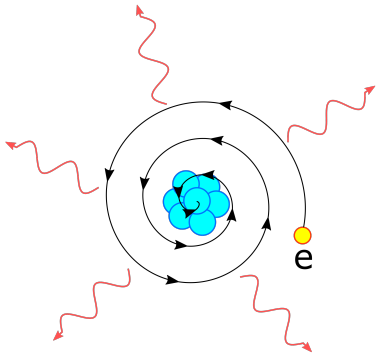
\includegraphics[width=0.33\textwidth]{iqis1_008}
\end{wrapfigure}

간단하게 핵을 중심으로 하여 고정된 궤도로 회전하는 전자의 모델을 취하자.
과학자들이 실감한 바 이는 전자라는 가속하는 전자가 거듭하여 방사선의
형식으로 에너지를 상실하고 핵에 이를 때까지 안쪽으로 나선 운동하는 모델이었다.
물리학자들은 전자 궤도가 안정적일 수 있는 근거와 이중 슬릿 실험 및 이외에도
무수한 현상을 설명하기 위해 확률의 계산법을 바꿔야 했다. 

물리학은 $P\in[0,1]$라는 확률 대신 \textbf{진폭}{\footnotesize amplitudes}
$a\in\mathbb{C}$를 사용하기 시작했다. 진폭은 양일 수도 음일 수도 있다. 더
일반적으로는 (실수와 허수 부분에 따라) 복소수일 수도 있다. \emph{양자역학의
핵심 주장}은 바로 격리된 계의 상태를 충분하게 설명하려면 측정할 적의 계로
발견되는 가능한 구성 각각에 대해 하나의 진폭을 부여해야 한다는 것이다.

\textbf{보른 규칙}{\footnotesize Born Rule}이 말하기를 특정 출력을 보는 확률은
진폭 절댓값의 제곱이다.

\begin{equation}{\label{eq:21}}
  P = |\alpha|^2=\textrm{Re}(\alpha)^2+\textrm{Im}(\alpha)^2.
\end{equation}

진폭은 복소수라는 사실이 진폭을 확률과 다르게 행동하게끔 하는지 보자. 진폭을
사용해 이중 슬릿 실험을 돌이키자.

\hfill

\hfill\parbox[t]{12cm}{
  $\alpha$는 스크린상 특정 지점에 안착하는 광자의 총 진폭,\\
  $\alpha_1$은 오직 1번 슬릿만 개방되었을 때 안착하는 광자의 진폭,\\
  $\alpha_2$는 오직 2번 슬릿만 개방되었을 때 안착하는 광자의 진폭이라고 하자.
}

\hfill\break

\noindent확률론에 빗대 다음을 취한다.
\begin{equation}
  \alpha = \alpha_1+\alpha_2.
\end{equation}
그런 다음 보른 규칙 \ref{eq:21}에서 다음을 취한다.
\begin{equation}
  P = |\alpha|^2=|\alpha_1+\alpha_2|^2=|\alpha_1|^2+|\alpha_2|^2+
  \alpha_1^*\alpha_2+\alpha_1\alpha_2^*.
\end{equation}
가령 $\alpha_1=1/2, \alpha_2=-1/2$일 때 두 슬릿 모두 개방되었다면 $P=0$이라고
확인할 수 있지만 하나의 슬릿만 개방된 경우 $P=1/4$다. 이 현상을
\textbf{간섭}{\footnotesize interference}이라고들 한다.


\newpage
그리하여 핵으로 나선 운동하지 않는 전자를 정당화하기 위해 말할 수 있는 바,
맞다. 전자가 그런 꼴을 보이는 경로는 여럿 있다. 하지만 어떤 경로는 양의 진폭을
지니며 다른 경로는 음의 진폭을 지닌다. 잇따라 이들 경로는 서로를 소거한다. 

\hfill

\hfill\parbox[t]{9cm}{\textcolor{gray}{\itshape 이 강의에서 다루지 않을 
물리학으로 진폭이 서로 소거하지 않는 확률은 이산 에너지 준위{\footnotesize
discrete energy levels}를 유도한다는 사실을 확인할 수 있다. 이산 에너지
준위는 전자들이 자리할 수 있는 곳이다. 이산 에너지 준위라는 현상은 결과적으로
화학을 요청한다.}}

\hfill

\section{선형대수학으로 보는 확률론}

계의 상태와 격리계의 진화를 각각 벡터와 벡터 변환으로 모델링하기 위해 
\textbf{선형대수학}을 사용한다. 두 상태를 지닌 계에 대해 가장 간단한
경우로는 다음처럼 작성할 수 있다.

\begin{equation}
M \begin{bmatrix} a_1\\a_2 \end{bmatrix} = 
\begin{bmatrix} a_1'\\ a_2' \end{bmatrix}
\end{equation}
당장은 고전 확률론을 다루겠다. 동전을 하나 던진다고 하자. 각 가능성에 
확률을 배정하여 벡터로 모델링한다. $p = P(\textrm{앞})$, $q = P(\textrm{뒤})$.

\begin{equation}
  \begin{bmatrix}p\\q\end{bmatrix}\quad
  \begin{aligned}
    &p,q \geq 0 \\
    &p+q = 1
  \end{aligned}
\end{equation}

변환을 적용할 수도 있다. 이를테면 \underline{동전을 뒤집을 수 있다}.

\begin{equation}
  \begin{bmatrix} 0 & 1 \\ 1 & 0 \end{bmatrix}
  \begin{bmatrix} p \\ q \end{bmatrix} = 
  \begin{bmatrix} q \\ p \end{bmatrix}
\end{equation}

동전을 뒤집는다는 말은 동전이 앞\emph{이었던} 확률은 이제 동전이 뒤\emph{인}
확률이라는 뜻이다. 다음 같은 변환 행렬이 이해를 도울 수 있겠다.

\begin{equation}
  \begin{bmatrix}
    P(\textrm{앞}|\textrm{앞}) &P(\textrm{앞}|\textrm{뒤}) \\
    P(\textrm{뒤}|\textrm{앞}) &P(\textrm{뒤}|\textrm{뒤})
  \end{bmatrix}
\end{equation}
여기서 $P(a|b)$는 동전의 원래 상태가 ``$b$''인 경우 동전의 상태가 ``$a$''인 조건부 확률이다. 또한 \underline{동전을 공평하게 뒤집을} 수도 있다.

\begin{equation}
  \begin{bmatrix}
    \frac{1}{2} & \frac{1}{2} \\
    \frac{1}{2} & \frac{1}{2}
  \end{bmatrix}
  \begin{bmatrix}p\\q\end{bmatrix} =
  \begin{bmatrix}\frac{1}{2}\\\frac{1}{2}\end{bmatrix}
\end{equation}
이전 상태와 무관하게 이제는 모든 가능성이 동일하게 그럴듯하다는 뜻이다. 
동전을 뒤집는데, 앞이 나오면 다시 뒤집지만 뒤가 나오면
앞으로 돌린다고 하자.

\begin{equation}
  \begin{bmatrix}
    \frac{1}{2} & 1 \\ \frac{1}{2} & 0
  \end{bmatrix}
  \begin{bmatrix} p \\ q \end{bmatrix} = 
  \begin{bmatrix} q+\frac{p}{2} \\ \frac{p}{2} \end{bmatrix}
\end{equation}
\emph{말이 되는가?} 동전의 상태가 앞이라고 밝혀지면 또 공평하게 던진다.
그리하여 앞이라는 결과가 주어지면 이후 또 던질 때 앞이나 뒤가 나올 확률은
$\frac{1}{2}$이라고 알 수 있다. 즉 $P(\textrm{앞}|\textrm{앞})= P(\textrm{뒤}|
\textrm{앞})=\frac{1}{2}$이다. 그리고 아무리 앞으로 던져도 계속 다시 뒤로
뒤집으니 $P(\textrm{뒤}|\textrm{뒤})=0$이고
$P(\textrm{앞}|\textrm{뒤})=1$이다. 

\emph{그래서 변환으로는 어떤 행렬을 사용할 수 있는가?} 우선 \underline{모든
요소는 음이 아니어야} 하겠다 (왜냐하면 확률은 음일 수 없기
때문이다). 또 \underline{각 열은 합이 $1$이어야} 하겠다. 초기
확률의 합이 변환된 확률의 합과 일치해야 하기 때문이다 (즉 둘 다
$1$과 같아야 한다). 이들 조건을 만족하는 행렬은 \textbf{확률 행렬}{\footnotesize
Stochastic Matrix}이라고 부른다. 

이제 동전을 두 개 던지고 싶다. 아니면 차라리 비트가 두 개 있다고 하자. 
첫 번째 비트는 $a = P(0)$과 $b = P(1)$이다. 두 번째 비트는 $c = P(0)$과
$d = P(1)$이다.

\[
  \begin{matrix}{\scriptstyle0} \\ {\scriptstyle1} \end{matrix}
  \begin{bmatrix}a \\ b\end{bmatrix}\quad\quad
  \begin{matrix}{\scriptstyle0} \\ {\scriptstyle1} \end{matrix}
  \begin{bmatrix}c \\ d\end{bmatrix}
\]
두 벡터를 합병하려면 새 연산이 필요하다. 이른바 \textbf{텐서 곱}{\footnotesize
Tensor Product}이다.

\begin{equation}
  \begin{bmatrix}a\\b\end{bmatrix} \otimes \begin{bmatrix}c\\d\end{bmatrix} =
  \begin{bmatrix}P(00)\\P(01)\\P(10)\\P(11)\end{bmatrix} = 
  \begin{bmatrix}ac\\ad\\bc\\bd\end{bmatrix}
\end{equation}

가능한 4원소 벡터 전부 두 2원소 벡터의 텐서곱으로 나타날 수는 없다. 주의할
만한 사실이다. 가령 모순적으로 아래처럼 가정하자. 

\begin{equation}
  \begin{bmatrix}ac\\ad\\bc\\bc\end{bmatrix} = 
  \begin{bmatrix}\frac{1}{2}\\0\\0\\\frac{1}{2}\end{bmatrix}
\end{equation}
그렇다면 첫째와 마지막 방정식의 곱은 $(ac)(bd)=\frac{1}{4}$이라고 암시하는
반편 둘째와 셋째의 곱은 $(ad)(bc)=0$을 암시하여 모순이 잇따른다. 
이처럼 우변의 4원소 벡터는 두 2원소 벡터의 텐서곱으로 작성될 수 없다.

단일비트계에서 그랬듯 이중비트계의 확률변환도 확률행렬로 기술할 수 있다.
가령 첫 비트가 $1$이면 두 번째 비트를 뒤집고 첫 비트가 $1$이 아닌 경우
계에 아무것도 하지 않는다는 변환을 적용한다고 하자. 이를 성취하는
$4\times4$ 행렬이 방정식 \ref{eq:212}에 있다. 통제된 NOT 혹은 CNOT 행렬이라고
부른다. 양자컴퓨팅에서도 자주 나올 예정이다.  

\begin{equation}
  \textrm{CNOT } = 
  \begin{bNiceMatrix}[first-col, first-row]
    & \scriptstyle00 & \scriptstyle01 & \scriptstyle10 & \scriptstyle11 \\
    \scriptstyle00 & 1 & 0 & 0 & 0 \\
    \scriptstyle01 & 0 & 1 & 0 & 0 \\
    \scriptstyle10 & 0 & 0 & 0 & 1 \\
    \scriptstyle11 & 0 & 0 & 1 & 0
  \end{bNiceMatrix}
  \label{eq:212}
\end{equation}
CNOT 행렬을 다음 벡터에 적용한다고 하자. 다음 벡터는 계 하나를 나타내는데 여기서
첫 비트는 $\frac{1}{2}$ 확률로 0이거나 1이며 두 번째 비트는 항상 0이다.
\begin{equation}
  \begin{bmatrix}
    1 & 0 & 0 & 0 \\ 0 & 1 & 0 & 0 \\ 0 & 0 & 0 & 1 \\ 0 & 0 & 1 & 0
  \end{bmatrix}
  \begin{bmatrix}
    \frac{1}{2} \\ 0 \\ \frac{1}{2} \\ 0
  \end{bmatrix}
  = 
  \begin{bNiceMatrix}[first-col]
    \scriptstyle00 & \frac{1}{2} \\ \scriptstyle01 & 0 \\
    \scriptstyle10 & 0 \\ \scriptstyle11 & \frac{1}{2}
  \end{bNiceMatrix}
\end{equation}
지금 출력된 분포는 앞서 텐서곱으로 나타날 수 없다고 증명한 것이다! 이런 분포를
\textbf{상호연관}{\footnotesize correlated}되어 있다고 한다. 비트 하나를 학습하면 
또 다른 비트에 관해서도 알 수 있다. 이 경우 두 비트는 항상 상등{\footnotesize
equal}이다. $50\%$ 확률로 둘 다 $0$이고 $50\%$ 확률로 둘 다 $1$이다. 그리하여
CNOT 행렬은 \emph{상호관계{\footnotesize correlations}를 만들}
수 있다고 알 수 있다.

양자역학은 본질적으로 똑같은 과정을 거쳐 벡터로 상태를 모델링하는데 \emph{딱
하나 다른 바,} 확률 대신 진폭을 사용한다. 양자 상태를 표현하는 벡터변환은 
행렬로 기술할 수 있다.
\begin{equation}
  \begin{bmatrix} & & \\ & U & \\ & &\end{bmatrix}
  \begin{bmatrix}a_1\\a_2\\a_3\end{bmatrix}=
  \begin{bmatrix}b_1\\b_2\\b_3\end{bmatrix}
\end{equation}
여기서는 벡터 요소의 합 대신 진폭 제곱 $\sum_{i=1}^3 |a_i|^2 = \sum_{i=1}^3
|b_i|^2 = 1$의 합을 보존한다. (보른 규칙) 방정식 \ref{eq:21}이
암시하듯 결과 확률의 합은 1이기 때문이다. 이런 행렬을 \textbf{유니터리
행렬}{\footnotesize Unitary Matrices}이라고 부른다. 다음 강에서는 
유니터리 행렬의 성질과 더불어 양자 상태를 다루기 위한 기본적인
수학 규칙을 훨씬 더 디테일하게 그리겠다.
\chapter{양자역학의 기본 규칙}
\section{양자 상태와 켓 표기}
\emph{양자 상태}는 (정확히 말해 ``순수 상태''는) 양자계의 상태를 묘사하는
$\mathbb{C}^N$상의 단위 벡터다. 이론적으로는 차원 $N$이 무엇이든 될 수 있다. 
물리학 강좌라면 위치 혹은 운동량 상태 같은 무한 차원 양자 상태를
다루겠지만 우리는 이산 계를 고수할 것이다. (말하자면 관측할 때면
오직 유한히 많은 결과만 있을 수 있다는 뜻이다) 

\hfill

\hfill\parbox[t]{9cm}{\itshape\textcolor{gray}{\underline{우주가 가장 기본적인
  수준에서 이산이나 연속으로 존재하는} \underline{광경에 대해 양자역학은 
  무슨 말을 할 수 있는가?} 양자역학은 이상한 하이브리드식 그림을 내놓는다.
  단순한 2차원계이더라도 가능한 양자 상태의 연속체가 존재하지만, 모든
관측은 이산적인 결과를 내놓는다. $[\alpha, \beta]^{\top}$라는 두 진폭으로
이루어진 계는 ($|\alpha|^2+|\beta|^2=1$이라는 제한을 두더라도) 
불가산적으로 무한하게 많은 가능한 상태를 지닌다. 그렇지만 고전 확률론으로 
상태를 나타내더라도 참이라는 사실에 유의하라. 고전과 양자라는 두 경우 모두에
대해 유한 차원 계를 고수하는 이상 연속체는 절대 직접적으로 관측되지
않는다. 다만 연속체는 이산적인 결과의 확률을 계산할 때만 쓰일 뿐이다.}}

\hfill\break

\textbf{큐비트}{\footnotesize qubit}는 가장 간단하고 흥미로운 양자계다.
(``$0$''과 ``$1$''이라는 레벨로 나타내는) 2레벨계{\footnotesize two-level
system}로 $0$에 대한 진폭과 $1$에 대한 진폭을 지닌다.

\hfill

\hfill\parbox[t]{9cm}{\itshape\textcolor{gray}{$1$레벨 양자계는 그냥 $[1]$이겠다.
그닥 흥미롭지 않다!}}

\hfill

폴 디락{\footnotesize Paul Dirac}이 도입한 표기를 따라 양자 상태 벡터는
이른바 \textbf{켓 표기{\footnotesize Ket Notation}}로 작성한다. 
\[
  \begin{bmatrix}\alpha\\\beta\end{bmatrix} 
  = \alpha\ket{0}+\beta\ket{1}=\ket{\psi}.
\]
$\ket0=\begin{bmatrix}1\\0\end{bmatrix}, \ket1=\begin{bmatrix}0\\1
\end{bmatrix}$이다. 일반적으로 양자 상태를 지시할 때는 $\ket{\psi}$를 종종
사용하겠다.

\emph{왜 켓 표기를 사용하는가?} 실용적으로 큰 이점 하나를 꼽는다면 (대다수 진폭이
$0$인) 아주 희소한 행렬{\footnotesize sparse vectors}이 빈번하다는 것이다.
켓 표기는 당장 화두인 값만 표현하기 쉽도록 한다.

\hfill

\hfill\parbox[t]{9cm}{\itshape\textcolor{gray}{사실 그냥 편하자고 도입하는
형식주의다. 켓 표기에 뭐든 넣을 수 있다. 자, 켓 표기 속 슈뢰딩거의 고양이다.
$\frac{1}{\sqrt2}\left(\ket{\twemoji[scale=.4]{grinning cat with smiling eyes}}
  +\ket{\twemoji[scale=.4]{crying cat}}\right)$}}
\end{document}
